
\documentclass[conference]{IEEEtran}

\usepackage{cite}
\usepackage{listings}
%\usepackage{booktabs}
\usepackage{color}
\usepackage{balance} % Helps to balance out text on last page
\usepackage{url}
\usepackage{times} % Used for formatting formatting url footnotes
\urlstyle{same} % Used for formatting formatting url footnotes


\usepackage{graphicx} % Including images



\lstset{ %
language=,                % Make language be nothing
basicstyle=\footnotesize,       % the size of the fonts that are used for the code
%numbers=left,                   % where to put the line-numbers; possible values are (none, left, right)
%numberstyle=\tiny\color{gray}, % the style that is used for the line-numbers
stepnumber=1,                   % the step between two line-numbers. If it is 1 each line will be numbered
numbersep=-3pt,                  % how far the line-numbers are from the code
backgroundcolor=\color{white},  % choose the background color. You must add \usepackage{color}
showspaces=false,               % show spaces adding particular underscores
showstringspaces=false,         % underline spaces within strings
showtabs=false,                 % show tabs within strings adding particular underscores
%frame=single,           % adds a frame around the code
tabsize=2,          % sets default tabsize to 2 spaces
captionpos=b,           % sets the caption-position to bottom
breaklines=true,        % sets automatic line breaking
breakatwhitespace=false,    % sets if automatic breaks should only happen at whitespace
escapeinside={\%*}{*)}          % if you want to add a comment within your code
}







\newcommand{\todo}[1]{\textcolor{cyan}{\textbf{[#1]}}}
\newcommand{\sam}[1]{\textcolor{red}{{\it [Sam says: #1]}}}
\newcommand{\dan}[1]{\textcolor{blue}{{\it [Dan says: #1]}}}

\begin{document}

\title{CAA: Concolic Analysis for Android}


\author{\IEEEauthorblockN{Daniel E. Krutz, Patrick McAfee
XXXX, and XXXX }
\IEEEauthorblockA{
%Software Engineering Department \\
Rochester Institute of Technology\\
One Lomb Memorial Drive, Rochester, NY, USA\\
\{dxkvse, pjm4439, xxxxx, xxxx\}@rit.edu}
}

\maketitle


\begin{abstract}

Mobile computing has become an important part of our everyday lives, and the Android operating system has grown to be the most popular mobile platform. Unfortunately, Android applications (apps) are not immune to many of the problems which plague all types of software, including bugs, security vulnerabilities and a wide range of other issues. Concolic analysis has been traditionally used to assist with these issues and have been used for a variety of purposes including software testing, code clone detection and security related activities. Concolic analysis is a hybrid software verification technique which performs symbolic execution along a concrete execution path.

We created a new concolic analysis tool for analyzing Android applications known as Concolic Analysis for Android (CAA). Built upon Java Path Finder (JPF), this tool performs concolic analysis on a raw Android application file or source code and provides output in a useful, and easily understandable manner. Our tool analyses the source code of an Android app using a complex wrapper to create entry points for the concolic analysis engine (JPF). The tool, usage instructions and source code is available on our project website:~\url{http://www.se.rit.edu/~dkrutz/CAA/}.  \todo{create website}


\end{abstract}
\IEEEpeerreviewmaketitle


\section{Introduction}

Android has grown to become an extremely popular mobile platform with its apps allowing the user to perform a multitude of activities ranging from banking to posting photos to Instagram. Concolic analysis has been traditionally used for software testing~\cite{Sen:2005:CCU:1081706.1081750}, security related activities~\cite{Chen:2014:CIB:2554850.2554875}, and code clone detection~\cite{Krutz_Sac15}. While there are a few conconolic analysis tools for Java, none are immediately compatible with Android source code since they are all are designed to explicitly work with a Java jar outside a framework, frequently requiring an explicit main method. Unmodified Java based concolic analysis tools such as JPF\footnote{\url{http://babelfish.arc.nasa.gov/trac/jpf/wiki}} or CATG\footnote{\url{https://github.com/ksen007/janala2}} will not work on Android applications since they lack a main method which is typically required of concolic analysis tools. We are proposing a new tool for performing Concolic Analysis on Android applications (CAA), which allows users to perform concolic analysis on Android application (.apk) and source files with ease, and without the need for a physical Android device or emulator. 

%%% Removed for space reasons 3/26
%%There were several hurdles we had to overcome in the creation of our tool. The Android SDK does not support calls to arbitrary main functions, so it is therefore necessary to provide a wrapper for a decompiled Android APK file in order to provide a single input to be used as the the root node for the concolic parser's tree. This leads to the second great problem with providing access, which is that Android applications are not designed to be run outside an Android runtime. The provided Android libraries for development are insufficient as they are only stub libraries. However, this obstacle was overcome through the use of Robolectric, a dynamic Android mocking mocking library which allows for coverage of Android code paths.

CAA is comprised of seven primary steps: (1) Unpacking the Android application (2) Conversion of apk into Jar file (3) Analysis of entry points into the application (4) Wrapper for decompiled APK (5) Creation of configuration files for concolic analysis tool (6) Running JPF (7) Log output from JPF.

%%% Removed for space reasons 3/26
%In the following work, we describe the need for our tool, provide details about the application and its design, and usage instructions. The source code of CAA, installation instructions and further results may be found on our website\footnote{\url{http://www.se.rit.edu/~dkrutz/CAA/}}.


\section{Related Work}
\label{sec: relatedwork}

There are an assortment of concolic tools which have been created for Java and C based applications. Some include JPF, CREST\footnote{\url{https://code.google.com/p/crest/}}, CATG and CUTE\cite{Sen:2005:CCU:1081706.1081750}. There are also several proposed techniques for applying concolic analysis to Android and mobile applications. Anand et al.\cite{Anand:2012:ACT:2393596.2393666} created a method known as ACTEve whose goal was to alleviate the path-explosion problem with concolic analysis. ACTEve is focused on event-driven applications such as smartphone applications and uses concolic analysis in order to generate feasible event-sequences for Android apps. Unfortunately this approach is often limited to short event sequences due to the resources required.

As with our tool, JPF-Android~\cite{vanderMerwe:2014:EPS:2557833.2560576} verifies Android apps using JPF. A primary benefit of this technique is that it allows Android applications to be verified outside of any emulator using JPF. While this work is profound, it differs from our tool in that it does not use concolic analysis to perform model checking and produces far different output than our tool. Mirzaei et al.\cite{Mirzaei:2012:TAA:2382756.2382798} described a process of testing Android applications through symbolic execution using custom Android libraries for JPF and simulated events through program analysis. While this work was substantial, it does not discuss the use of concolic analysis and does not appear to have been publicly released as a fully functional tool.


%While none use concolic analysis, there are a plethora of powerful testing tools for Android apps. Dynadroid\footnote{\url{https://code.google.com/p/dynadroid/}} is a tool for creating inputs to unmodified Android apps.  Google even provides its own testing framework to developers\footnote{\url{http://developer.android.com/tools/testing/testing_android.html}}.


\section{Concolic Analysis}
\label{sec: concolicanalysis}

%%% Removed for space reasons 3/26
%Symbolic analysis is used to execute a program using symbolic inputs utilizing~\emph{path conditions} which are updated whenever a branch of the source code is executed. Symbolic values are used in place of actual, concrete values to represent the variables of the target application~\cite{King:1976:SEP:360248.360252,Cadar:2011:SES:1985793.1985995}. Symbolic analysis has been traditionally used for testing applications finding defects and assisting with the creation of unit tests. A primary drawback of symbolic analysis is the~\emph{path explosion} problem which is the creation of a large, or impractical number of paths for symbolic analysis to follow.


Concolic analysis is the combination of concrete and symbolic values to analyze software and has been used for testing, assisting with unit test creation, identification of software clones, and the discovery of security vulnerabilities~\cite{Sen:2005:CCU:1081706.1081750, Godefroid_automatedwhitebox, 6671332, Krutz_Sac15}. Concolic analysis was introduced by Sen et al.~\cite{Sen:2005:CCU:1081706.1081750} in 2005, and has an advantage over symbolic analysis since the combination of concrete and symbolic values can be used to simplify constraints and precisely reason about complex data structures~\cite{4222603}.

When an application is executed using concolic analysis, the execution path along with symbolic constraints are stored in the~\emph{path condition}. An execution branch is then selected from this path condition which is then provided to the constraint solver to be verified for legitimacy. If correct, concrete test inputs are then used to create a new achievable application path. However, if the new path is found to be unachievable, another application path is then selected. Using this process, concolic analysis attempts to traverse as many paths of the application as possible while limiting the path explosion problem through its use of concrete values~\cite{Jaffar:2013:BCT:2491411.2491425}.




\section{Concolic Analysis for Android Tool}
\label{sec: caa}

The core of CAA is based on linking several previously existing tools together in order to provide a framework where concolic analysis can be run with a tool. CAA is designed as an automated toolchain, utilizing other disparate tools to do the more complex tasks.  There are four primary tools that are crucial to CAA. The first two of these, Dex2Jar\footnote{\url{https://code.google.com/p/dex2jar/}} and Apktool\footnote{\url{https://code.google.com/p/android-apktool/}}, are Android application manipulation tools described in greater contextual detail below in the design section. The third is Robolectric\footnote{\url{http://robolectric.org/}} which is a library specially designed to stub and mock out the Android runtime when testing a project outside of a runtime.  In the context of this project, it is used to grant access to code paths during concrete execution that other would be unreachable without that framework.
The fourth tool is the most critical, as it is the tool used to run the actual concolic analysis. The tool that has been selected for this purpose is JPF.  While there are other tools that provide this functionality against vanilla jars, such as jCUTE\footnote{\url{http://osl.cs.illinois.edu/software/jcute/}} or CATG, JPF is a best fit for this project, particularly its Symbolic optional module with includes the actual concolic analysis. Firstly, it is affiliated with NASA and is actively supported with a robust development community, which was critical to this project's development. A critical feature found here that other tools did not include was the ability to configure a flexible classpath at runtime with multiple directories. This functionality was required for the dynamic compilation described in the design portion of this paper.

In the following sections, we will provide an overview of CAA's architecture, usage instructions, output and results. 

\subsection{Overview of Architecture}


\begin{figure*}[ht!]
\centering
%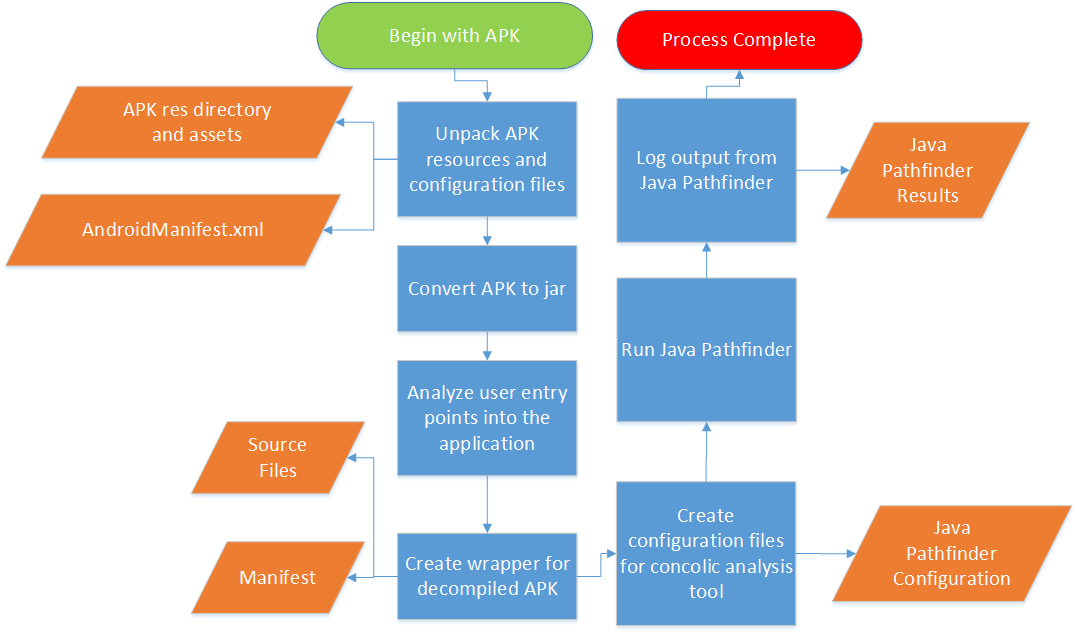
\includegraphics[width=1.0\textwidth]{images/workflow.png}
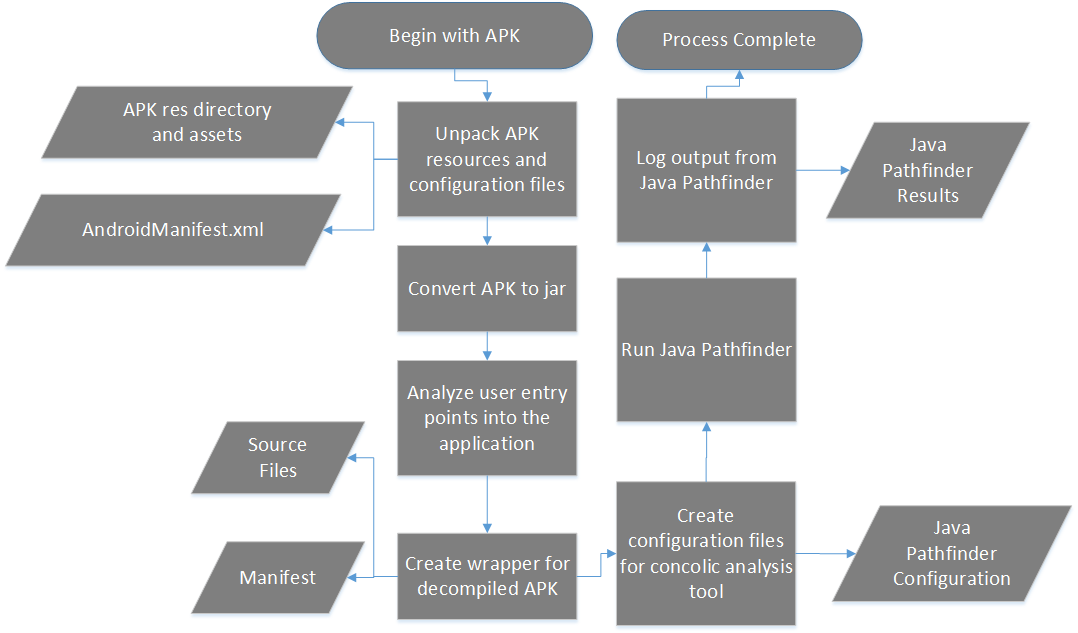
\includegraphics[width=14cm,height=10cm,keepaspectratio]{images/workflow_grey.png}
\caption{CAA Workflow}
\label{fig:workflow}
\end{figure*}


CAA accepts a path to an APK and executes a linear series of steps to provide the results of concolic analysis.  A high level overview of the process is described below and is shown in Figure~\ref{fig:workflow}.

\begin{enumerate}

 \item Unpack APK resources and configuration files
 \item Convert APK .dex files to Java .class files
 \item Analyze user entry points into the application
 \item Create wrapper for decompiled APK
 \begin{enumerate}
 	\item Create java source files for wrapper from templates
 	\item Fill templates with entry point information and calls
 	\item Compile the wrapper
 \end{enumerate}
 \item Create configuration files for concolic analysis tool
 \item Run JPF
 \item Log output from JPF
 \end{enumerate}

The first step of the process uses Apktool, a Java utility for decompiling Android applications. This tool extracts the UI resources and other assets from the jar, as well as decrypting the AndroidManifest.xml file.  These assets and configs are crucial for Robolectric to run correctly later in the process.  All the extracted files are placed in a special directory for later manipulation along with a copy of the targeted APK file.  All further modification is done in this directory.

The second step utilizes Dex2Jar, a utility for decompiling APK files into standard Java jars. The jar format is required for later compilation and manipulation by CAA. It exposes access to the internal code in a way that standard Java tools can easily work with.  It can also provides readable source, an invaluable resource during development.  This jar is also stored within the spawn directory.
The third step is instrumented by CAA.  This involves analyzing the provided source from the generated jar file. Through the use of reflection, each class is dynamically loaded and analyzed for known inputs, such as an OnCreate method of an Activity. A blocklist is used to prevent excessive automated analysis of the Android libraries themselves, which are dynamically loaded to a custom classpath so that proper matching can happen.  The types of inputs found are used to determine what functions need to be called and what kind of data they need to be sent by CAA and JPF.

The fourth and most complex step creates a custom wrapper jar against the created jar. Several template files are used to create raw Java source files with tokens.  These tokens are replaced by a source writer in CAA, which interprets the analysis from the previous step.  Calls to supported functions the framework or user would trigger manually are automated in the source files.  There are two .java files and and a manifest file created from this process, as well as a .jpf file. The first Java file is a wrapper that makes all of the aforementioned calls to the jar converted from the APK file and wraps those calls in a single function as a JUnit test. Robolectric, the Android mocking library being used, operates as a JUnit TestRunner and thus the wrapper function must be a test to utilize the mocks. The second Java file is the wrapper runner whose purpose is load the wrapper's tests into JUnit and fire them from inside a single entry point. This entry point is then exposed to JPF and indirectly provides access to the underlying functions from the APK file.  The final file is a custom manifest that references all dependencies as well as the jar converted from the APK.  The newly created Java source and manifest are packaged into a custom wrapper jar to be used in the next step of the process.

The fifth and sixth steps build on part of the fourth. During the creation of files from templates, a .jpf file is created. This .jpf file is used by JPF to store arguments to pass to the concolic tool. In particular, this stores the targeted entry function provided by the wrapper jar, the functions that should have the analysis run on them, and the settings to enable concolic analysis. Finally, the output generated by the tool is saved for the user. A small example portion of the output is shown in Listing~\ref{lst:concolicoutput}, while more complete results may be found on the project website.

\begin{lstlisting}[label=lst:concolicoutput, caption=Example Concolic Output]
8 : checkcast
11 : putfield java.util.HashMap.table
14 : aload_0
15 : iconst_0
16 : putfield java.util.HashMap.hashSeed
19 : aload_0
20 : aconst_null
21 : putfield java.util.HashMap.entrySet
24 : iload_1
\end{lstlisting}



\subsection{Usage Instructions}

The tool is available from our project website and our public GitHub Repo\footnote{\url{https://github.com/ConcolicAnalysisAndroid/}}. Once downloaded and installed using the instructions provided in these locations, the tool may be used via the following command:~\emph{``java -jar CAA-1.0.0.jar \-apk \$PATH\_TO\_APK''} where \$PATH\_TO\_APK is the relative or absolute path to the apk file to be analyzed.  A directory named ``spawn'' will be created where several temporary artifacts of the process will be created. Results will be logged in a created directory named ``results'' in the form of text files named as ``\$APK\_FILENAME.jpfout.txt.'' The results directory is located in the same directory as the application. A thorough example set of instructions on running the tool may be found on the project website.


%An example screen showing CAA is shown in Listing~\ref{lst:concolicoutput}.

\begin{figure}[ht!]
\centering
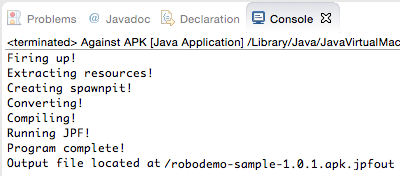
\includegraphics[width=0.45\textwidth]{images/CAA_Eclipse_small.png}
\caption{Example CAA Usage}
\label{fig:usingCAA}
\end{figure}


\section{Limitations \& Future Work}
\label{sec: limitations}

% Android function calls which require highly specific feedback require more targeted mocking than Robolectric can generically provide.

In its current form there are several limitations to CAA. The targeted coverage is limited to the activity lifecycle startup and is also limited by the intentional black box testing nature of usage with mocks. The primary issue with the black box nature of this application is that certain Android apps require highly specific data at certain intervals, such as when communicating with servers. Robolectric has no way of knowing what an app expects back from specific calls, and thus cannot correctly mock it out. Robolectric can only mock out more simple or common Android API calls. This may cause certain code paths to be excluded from coverage if specific results for calls are expected.

During the creation of tool, the Dalvik runtime was the the only Android runtime. Near the end of development, Android 5.0 was released using the ART runtime. Available APKS are currently theoretically compatible with both and are convertible by Dex2Jar. In the future, this may not be the case as there have been discovered incompatibilities and over time the Dalvik runtime will eventually be left behind.  This brings up the important caveat that CAA is limited by the tools it relies on and all of the ensuing quirks and issues associated with them.  A strong example of this exists in JPF where the development of CAA revealed several issues and bugs associated with that tool's implementation of reflection, some of which are still outstanding and affect the reliability of CAA.



The source writer can also be expanded to provide more coverage. For example, a filter for Android services could be added and the wrapper files could be compiled to target the launch and processing of these application parts. This example could be expanded upon as the Android SDK grows and changes, allowing new entry points and data sources to be covered. No significant amount of work has been done to compare CAA to any existing Android testing tools. Areas of comparison include analysis time, amount of code coverage, and precision \& recall of known errors.

%%% Removed for space reasons 3/26
%There are many improvements that can be made to CAA. A notable one is that CAA is limited to inefficiently processing one APK file at a time. The concurrent processing of multiple applications makes the usage of the tool more efficient and opens up the application to be more easily utilized by other tools.  An example of this would be to compare two similar apps and run heuristics on the generated output, which is a use case that led to the creation of this tool.



% What improvements can be made to this tool?
%	Code coverage
%	Use different concolic analysis engine or write our own
% Apply to other areas such as clone detection in Android applications and detecting repackaged Android applications
%       Take a look at where else CA has been traditionally used
%

%%% Removed for space reasons 3/26
%\section{Conclusion}
%\label{sec: conclusion}

%We have presented CAA, a tool that analyzes Android applications using concolic analysis. While there are numerous other testing tools for Android applications, and even some which use concolic analysis; this is the first known tool of its kind which is able to perform concolic analysis using only the source code of the Android application \todo{check to make sure that this is true}.

%%%%%% Removed for space reasons 3/26
%%%%CAA first extracts the source code of the application using existing tools including Apktool and Dex2Jar. Using reflection, CAA then dynamically loads the extracted Java class files looking for known inputs which are used in the customer wrapper, the most complex aspect of the system. These are used by JPF to perform concolic analysis on the app, and then generate the concolic output, which may be used by a variety of other applications.

%We have made the tool, source code, and usage instructions available on our project website and encourage others to use the tool not only for testing Android applications, but in their research as well.




%\end{document}  % This is where a 'short' article might terminate
\balance
\bibliographystyle{abbrv}
\bibliography{CA_Android_tool}

% That's all folks!
\end{document}



% Todo
% 	Create a website for the tool and make sure GH page is public
% 	Move the Tool to the head (top) of https://github.com/ConcolicAnalysisAndroid/


% Thoughts
%


% Tool demo: 3 page proposal
%	http://www.icsme.uni-bremen.de/cfp_tool.php


%%% Focus more on the wrapper aspect and that is what this is
% Maybe have the student listed 1st?